\section{Algebrotopologiset määritelmät}

Tässä työssä solmujen ominaisuuksien tutkimiseen tarvitaan topologisia työkaluja. Tämän osion päätarkoituksena on määritellä harvinaisia, solmuteorialle tyypillisiä konstruktioita ja peruskäsitteistö oletetaan lukijan hallitsemaksi.\footnote{Topologian peruskäsitteistöä tuntematonta lukijaa suositetaan perehtymään esimerkiksi tiiviiseen luentomuistiinpanoon \citep{koski2024topology} tai syvällisempään johdantoon \citep{Munkres2000}.} Algebrallisen topologian käsitteistössä seuraillaan Hatcherin \citep{Hatcher2002} kirjaa.

Tämä osio palvelee kahta tarkoitusta: putkiympäristön käsitteen kehittämistä sekä teknisempää todistusta siitä, että kahden homologisen $n$-pallon yhteen pujominen\footnote{Pujominen määritellään solmuja koskevassa kappaleessa ???} tuottaa homologisen $n$-pallon. Käyrän putkiympäristöä voi ajatella pienenä käyrää seurailevana täytettynä putkena. Homologisia palloja koskeva lause varmistaa, että kun kaksi eri avaruuksissa elävää solmua pujotaan yhteen, elää tulossolmu myös ``hyvänlaatuisessa'' avaruudessa.

Formaaleista muotoiluista kiinnostunut lukija voi tutustua osakappaleisiin tarkemmin, mutta niiden sivuuttaminen ei estä lainkaan myöhempiin kappaleisiin perehtymistä.
\subsection{Kimput}
Kuitukimppua voidaan pitää topologisten avaruuksien tulon $X\times Y$ yleistyksenä sikäli, että se sallii ``vääntyneen'' tulon. Vektorikimppu on kuitukimpun erityistapaus.
\begin{maaritelma}[Kuitukimppu]
    \emph{Kuitukimppu} on nelikko $(E,B,\pi,F)$, missä $E,B$ ja $F$ ovat topologisia avaruuksia ja $\pi:E\to B$ jatkuva surjektio, joka tyydyttää paikallisen triviaaliuden ehdon (alla). Sivu 386 alg. top. kirjasta.
\end{maaritelma}
Kuitukimpun pitää olla paikallisesti triviaali eli muistuttaa tavallista tuloa, mutta globaalisti sen geometria voi olla vääntynyt. Kuva~\ref{kuva:epätriviaali-torus-kuitukimppu} esittää epätriviaalisti vääntynyttä torusta. Siinä jokainen kuitu kierii toruksen pienemmän akselin ympäri viisi kertaa ennen lähtöpisteeseen palaamista ja kuvaan on piirretty kolme kuitua.
\begin{figure}
    \centering
    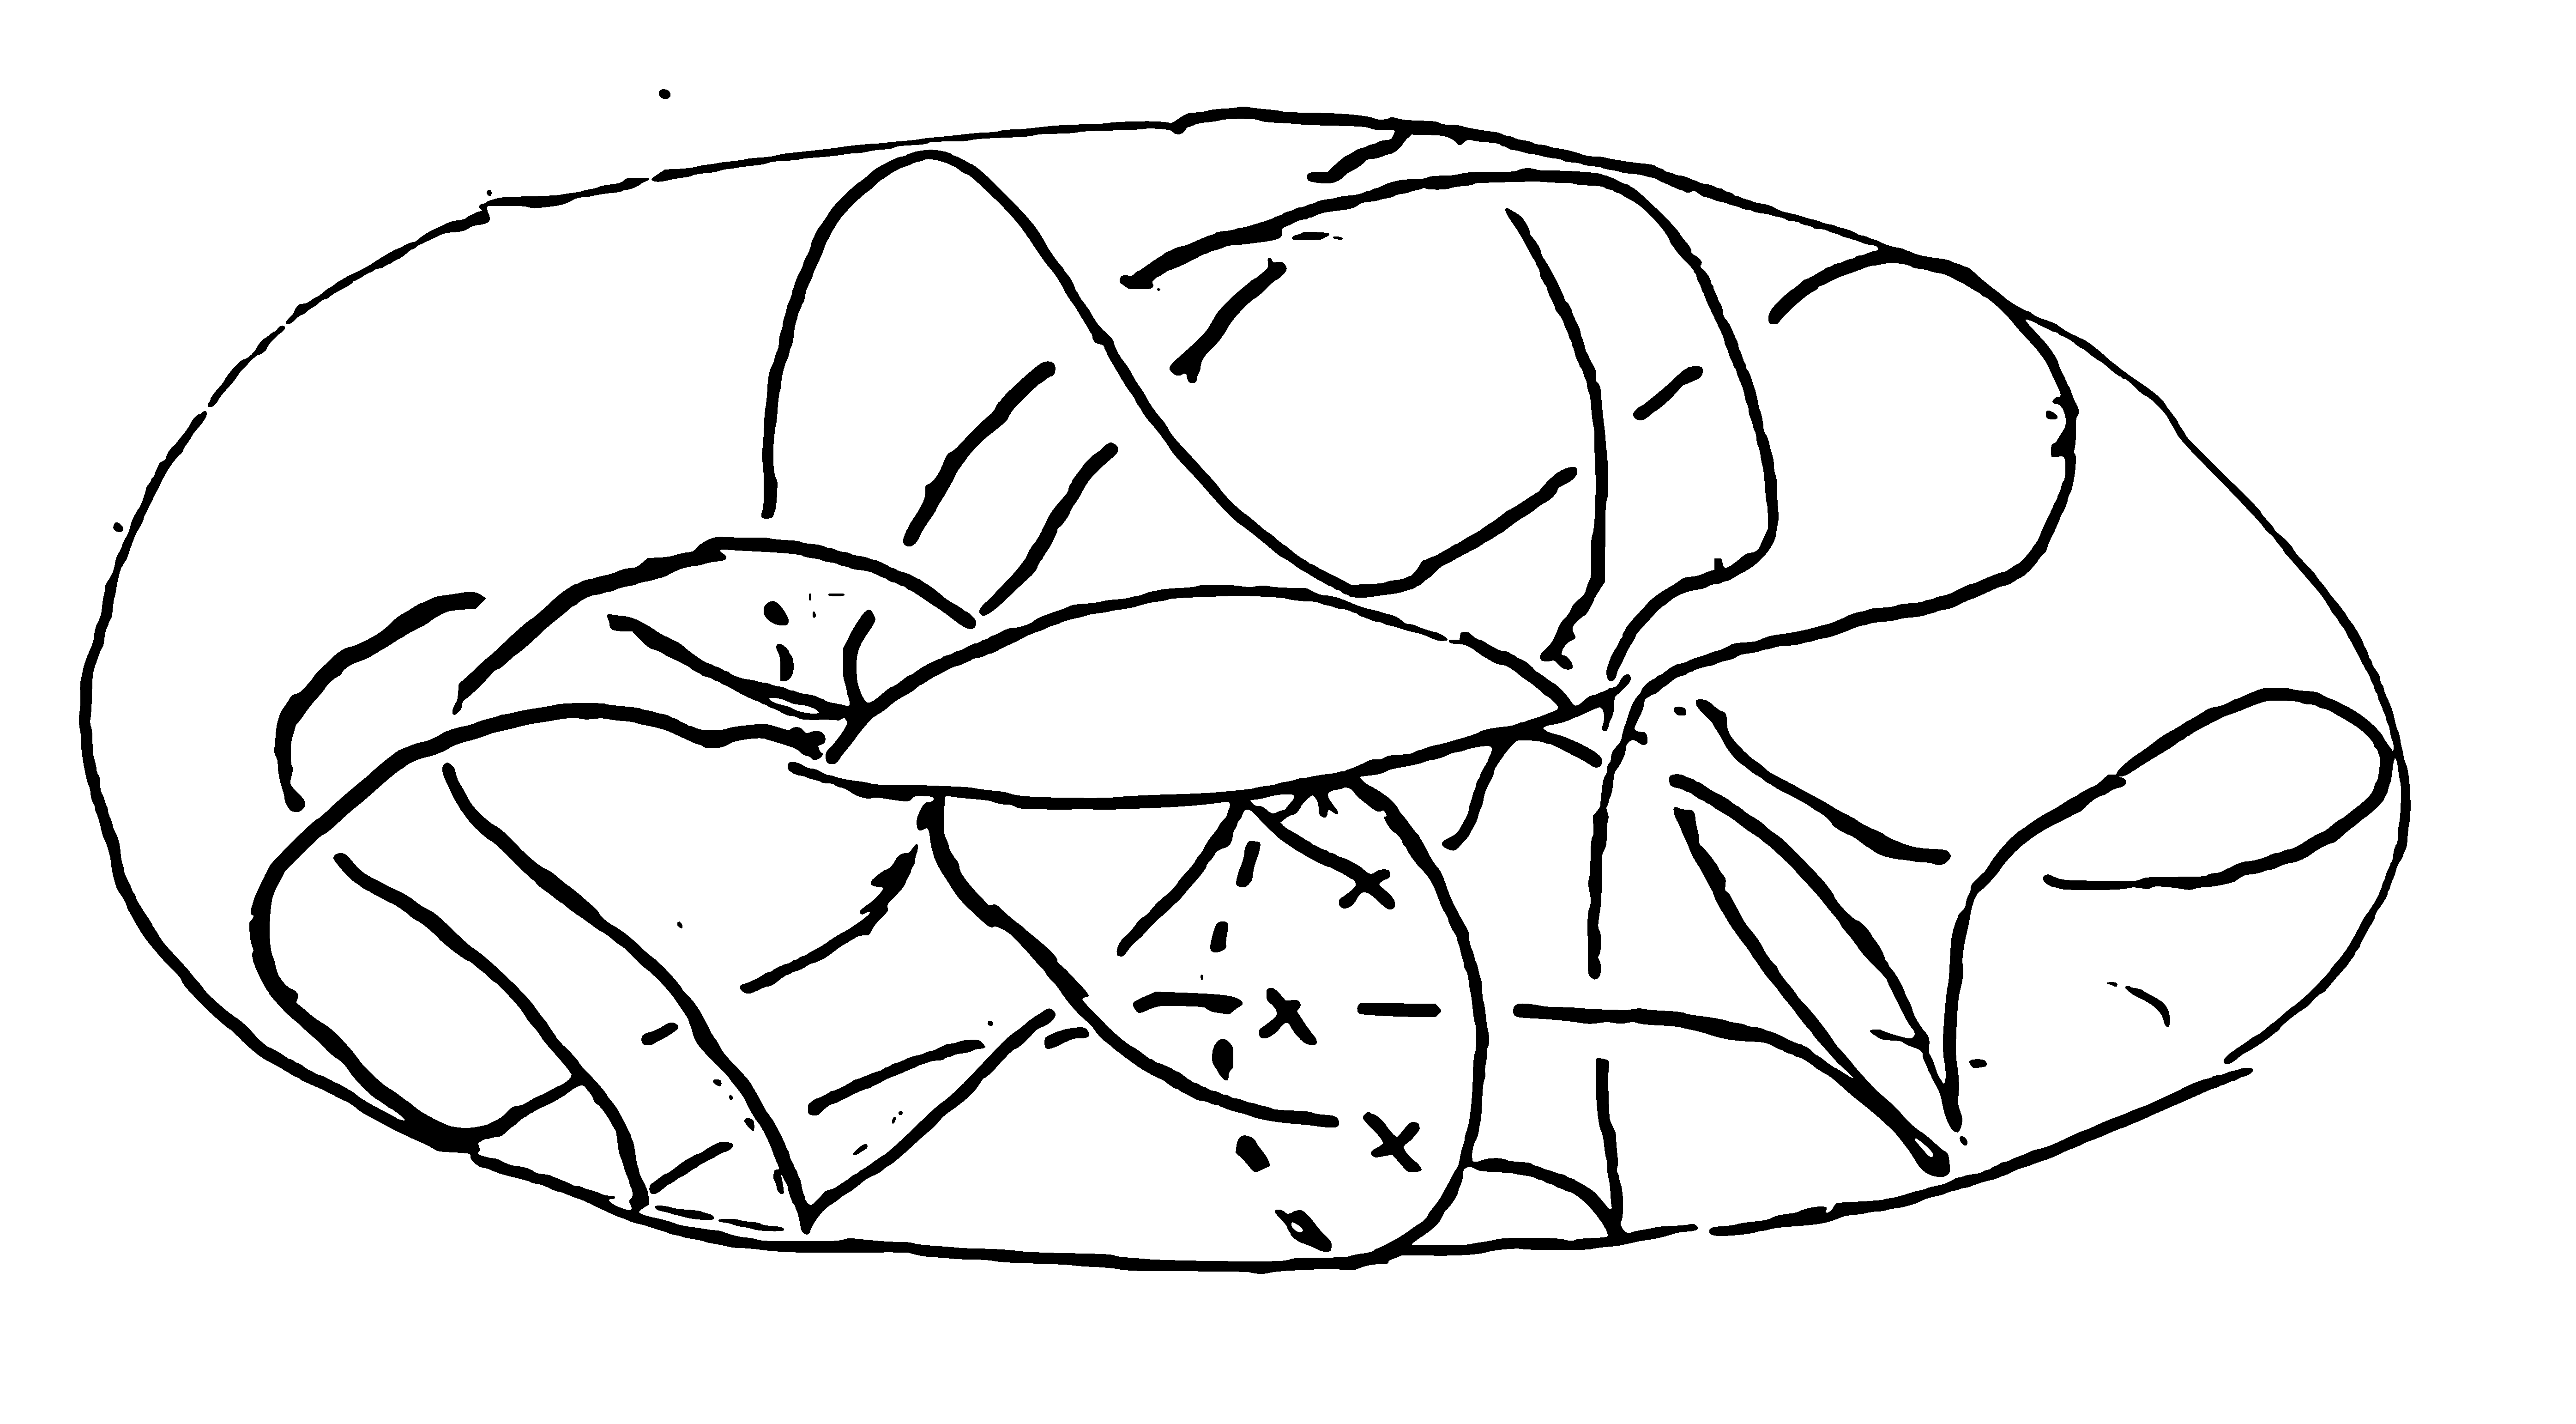
\includegraphics[width=0.5\textwidth]{figures/epätriviaali-torus-kuitukimppu.pdf}
    \caption{Epätriviaali torus, jossa kuidut ovat vääntyneitä.}
    \label{kuva:epätriviaali-torus-kuitukimppu}
\end{figure}
\begin{maaritelma}[Vektorikimppu]
    Olkoon $M$ topologinen avaruus. Asteen $k$ $\K$-\emph{vektorikimppu} $M$:n yli on jatkuvalla surjektiolla $\pi:E\to M$ varustettu topologinen avaruus $E$ siten, että 
    \begin{enumerate}
        \item kaikille $p\in M$ kuitu $E_p=\pi^{-1}(p)$ yli $p$:n voidaan varustaa $k$-ulotteisen $\K$-vektoriavaruuden rakenteella ja
        \item kaikille $p\in M$ on olemassa $p$:n ympäristö $U\subset M$ ja homeomorfismi $\Phi:\pi^{-1}(U)\to U\times\K^k$ siten, että
        \begin{itemize}
            \item $\pi_U\circ\Phi=\pi$ (jossa $\pi_U:U\times\K^k\to U$ on projektio) ja
            \item kaikille $q\in U$ $\Phi|_{E_q}$ on vektoriavaruusisomorfia $E_q\cong\{q\}\times\K^k\cong\K^k$.
        \end{itemize}
    \end{enumerate}
\end{maaritelma}
\begin{esimerkki}
    Esimerkiksi pallo ja sen tangenttikimppu muodostavat vektorikimpun $\pi:T\S^2\to\S^2$, jossa projektio määritetään $T_p\S^2\mapsto p$ eli pisteeseen, jossa tangenttiavaruus kiinnittyy palloon. Tässä jokainen kuitu voidaan varustaa 2-ulotteisella $\R$-rakenteella.
\end{esimerkki}
Pallo ja tangenttikimppu ovat esimerkkeji globaalisti triviaalista vektorikimpusta, jossa ei ole vääntöä. Möbius-nauha kuvassa~\ref{kuva:mobius-nauha} muistuttaa paikallisesti tuloa $\S^1\times I$, missä $I\subset\R$, mutta globaalisti se on vääntynyt.
\begin{figure}
    \centering
    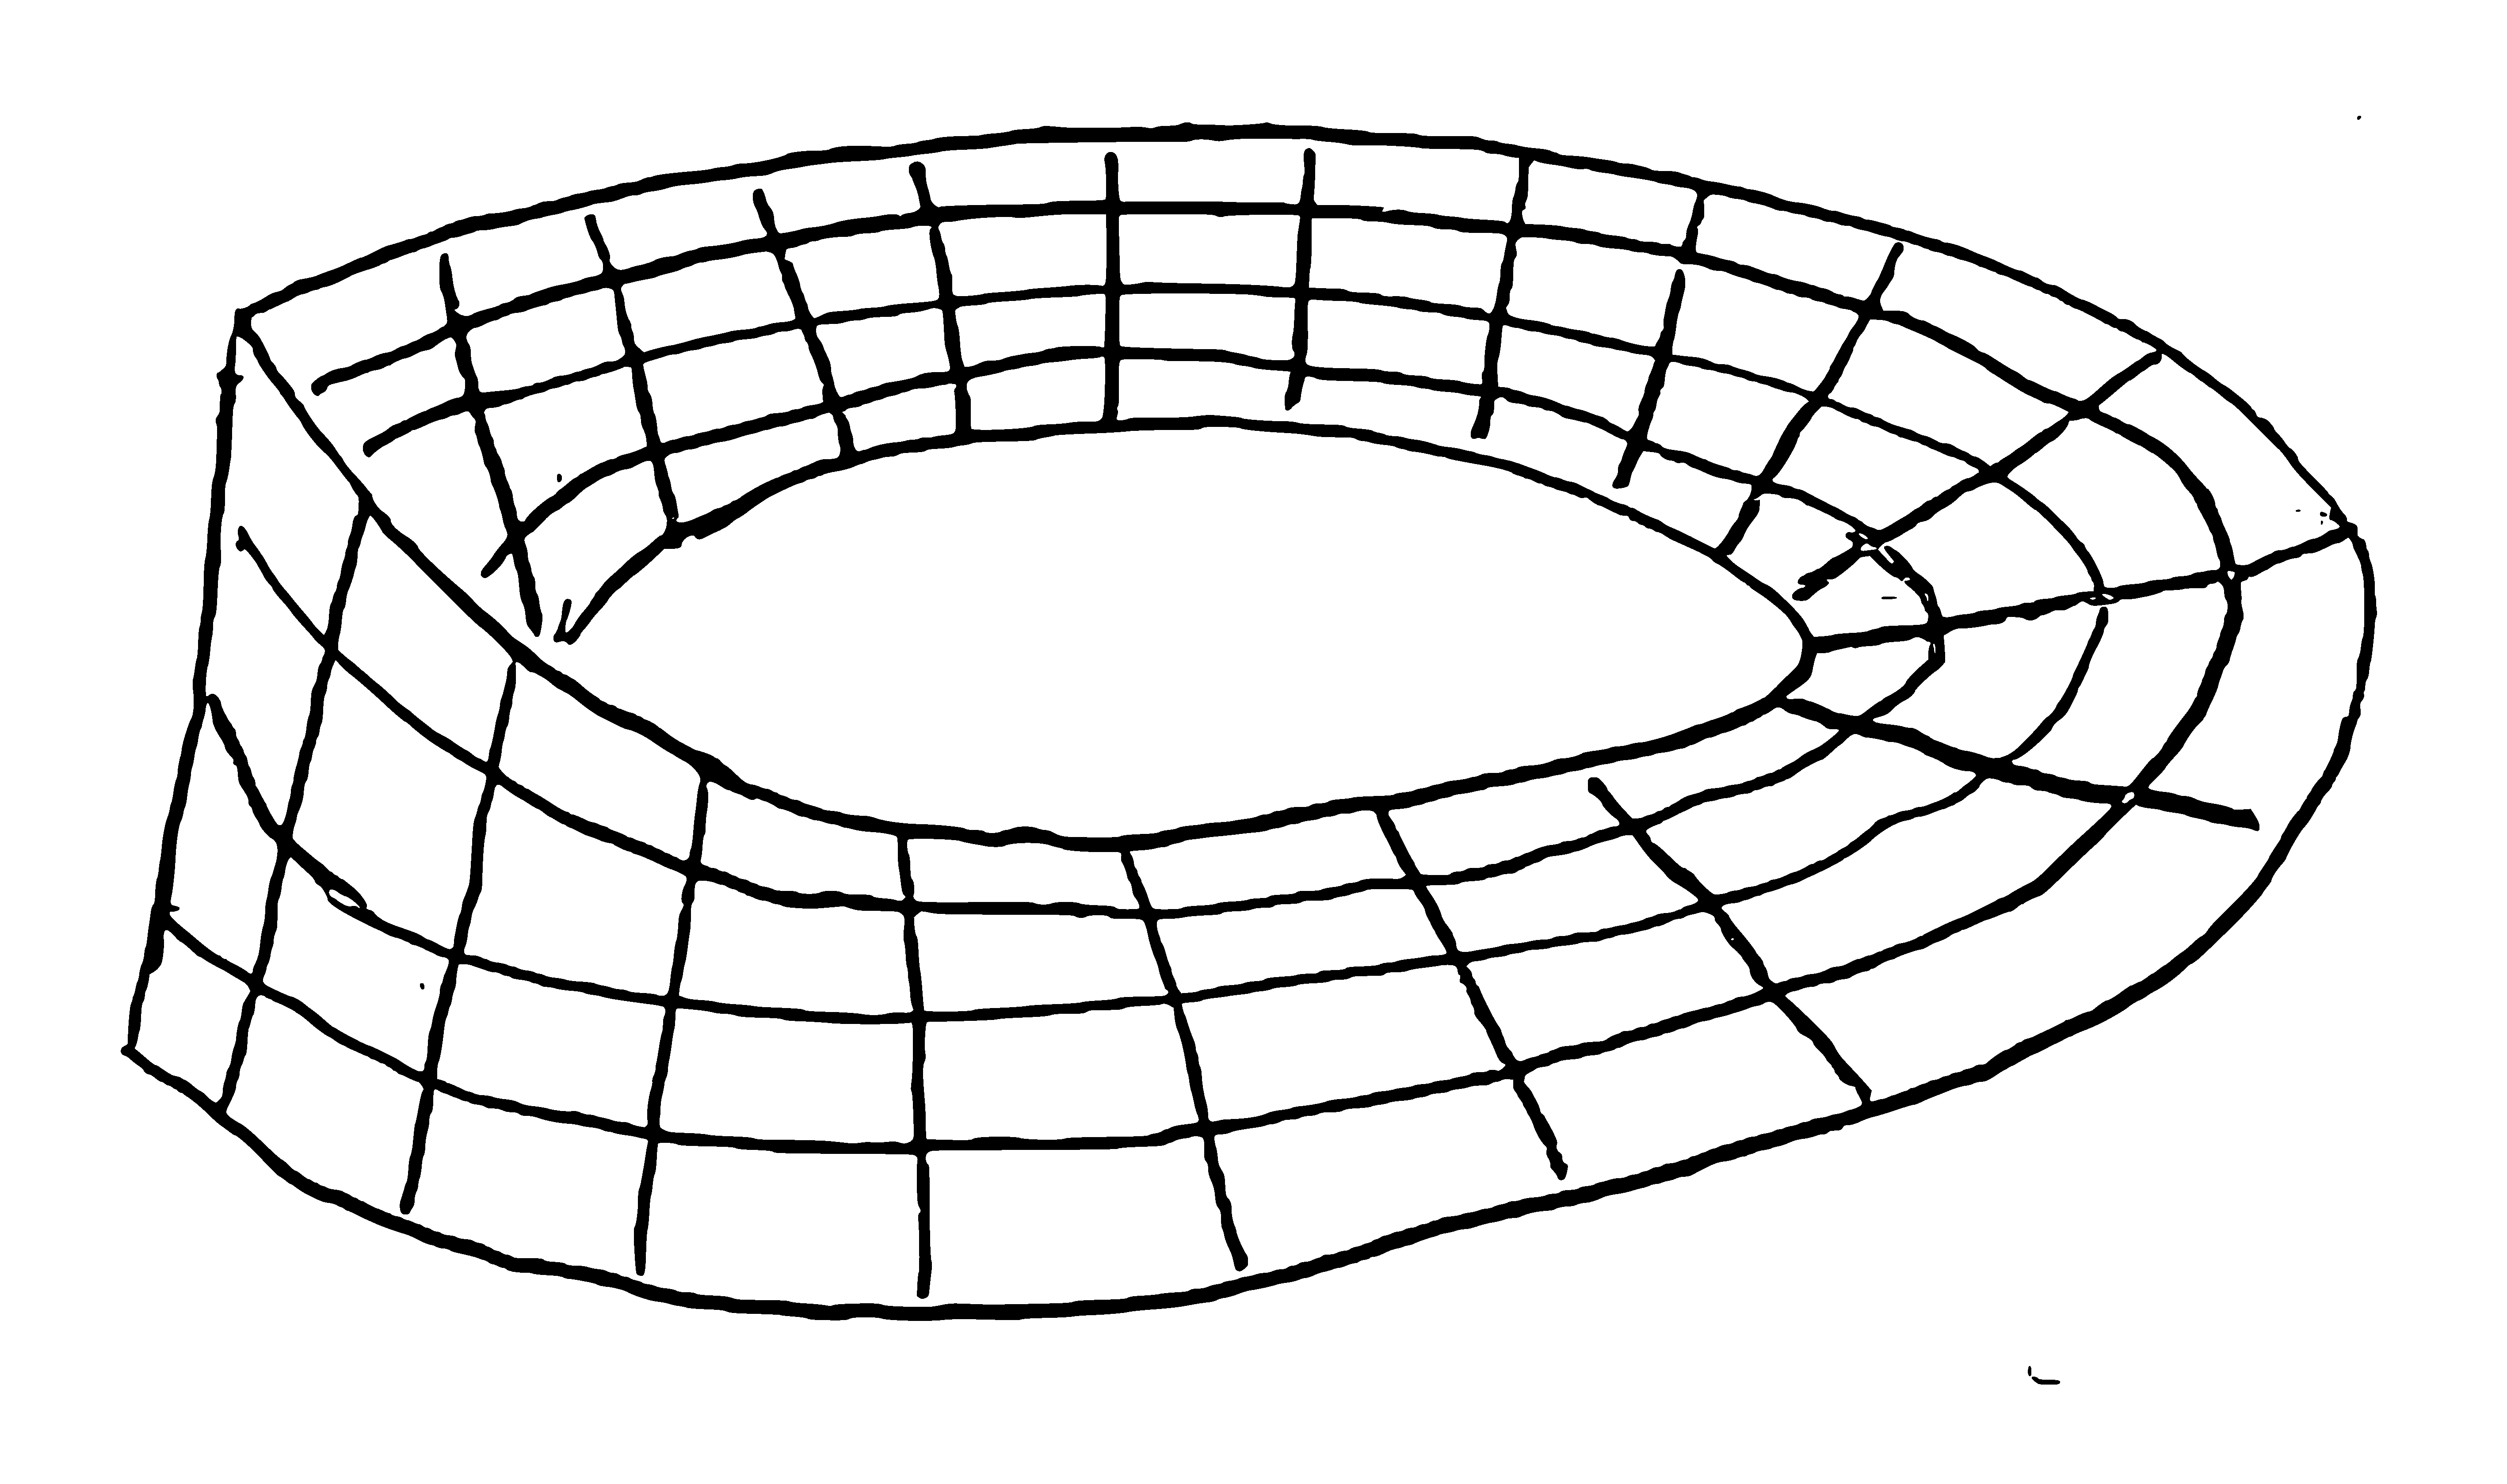
\includegraphics[width=0.5\textwidth]{figures/mobius-nauha.pdf}
    \caption{Möbius-nauha.}
    \label{kuva:mobius-nauha}
\end{figure}


\subsection{Kuidut}
Siinä missä kuitukimppu yleistää topologisen tulon, kuidutus yleistää kuitukimpun. Kuidutuskonstruktio on hankala käsittää ja se esitetään tässä pääosin vain myöhempää konstruktiota, putkiympäristöä, varten.
\begin{maaritelma}[Homotopinen nosto-ominaisuus]
    Kuvaus $\pi:E\to B$ tyydyttää \emph{homotopisen nosto-ominaisuuden} avaruudelle $X$, jos
    \begin{itemize}
        \item kaikille homotopioille $g:X\times[0,1]\to B$ ja
        \item kaikille kuvauksille $\tilde g_0:X\to E$ nostaen $g_0=g(\cdot,0)$:n, eli $p\circ\tilde g_0=g_0$,
    \end{itemize}
    on olemassa homotopia $\tilde g:X\times[0,1]\to E$ nostaen $g$:n (eli $g=p\circ\tilde g$) niin, että $\tilde g_0=\tilde g|_{X\times\{0\}}$. Kommutoiva kaavio havainnollistaa tilanteen:
    \begin{equation}
        \begin{tikzcd}
            X\times\{0\} \arrow[r, "\tilde g_0"] \arrow[d, hook] & E \arrow[d, "\pi"] \\
            X\times[0,1] \arrow[ur, dashrightarrow, "\tilde g"] \arrow[r, "g"] & B
        \end{tikzcd}
    \end{equation}
\end{maaritelma}
\begin{maaritelma}
    \emph{Kuidutus} on kuvaus $\pi:E\to B$, jolla on homotopinen nosto-ominaisuus kaikkien avaruuksien $X$ suhteen.
\end{maaritelma}
\begin{maaritelma}
    Olkoon $\pi:E\to B$ kuidutus. Kuidutus on \emph{paikallisesti triviaali}, jos kaikille $x\in B$ on olemassa avoin ympäristö $U\subset B$ siten, että 
    \begin{equation*}
        \pi^{-1}(U)\approx U\times F.
    \end{equation*}
\end{maaritelma}
\begin{maaritelma}
    Jos $E$ on pohja-avaruuden $B$ kuitukimppu $\pi:E\to B$, niin \emph{kuitukimpun sektio} on jatkuva kuvaus $\sigma:B\to E$ siten, että $\pi\circ\sigma=\text{id}_B$.
\end{maaritelma}

\subsection{Putket}
\begin{maaritelma}
    Olkoot $S,M$: $S\subset M$ sileitä monistoja. $S$:n \emph{putkiympäristö} $M$:ssä on pari $(\pi, J)$, jossa $\pi: E\to S$ on vektorikimppu ja $J:E\to M$ on sileä kuvaus, siten että
    \begin{itemize}
        \item $J\circ0_E=i$, $i$ on upotus $S\hookrightarrow M$ ja $0_E$ nollasektio
        \item on olemassa avoimet joukot $U\subset E$, $V\subset M$ siten, että $0_E[S]\subset U$ ja $S\subset V$ niin, että rajoitus $J|_U$ on diffeomorfismi.
    \end{itemize}
\end{maaritelma}
Yksinkertainen esimerkki saadaan käyrästä $\R^3$:ssa. Sen putkiympäristö on käyrää seuraileva kolmiulotteinen mato, jonka poikkileikkaukset ovat tasojoukkoja, joiden muoto vaihtelee, mutta käyrän suuntaisesti aina sileästi. Putkiympäristön läpileikkaus ei välttämättä ole ympyrälevyn mallinen. Esimerkki kuvassa~\ref{kuva:putkiympäristö}.
\begin{figure}
    \centering
    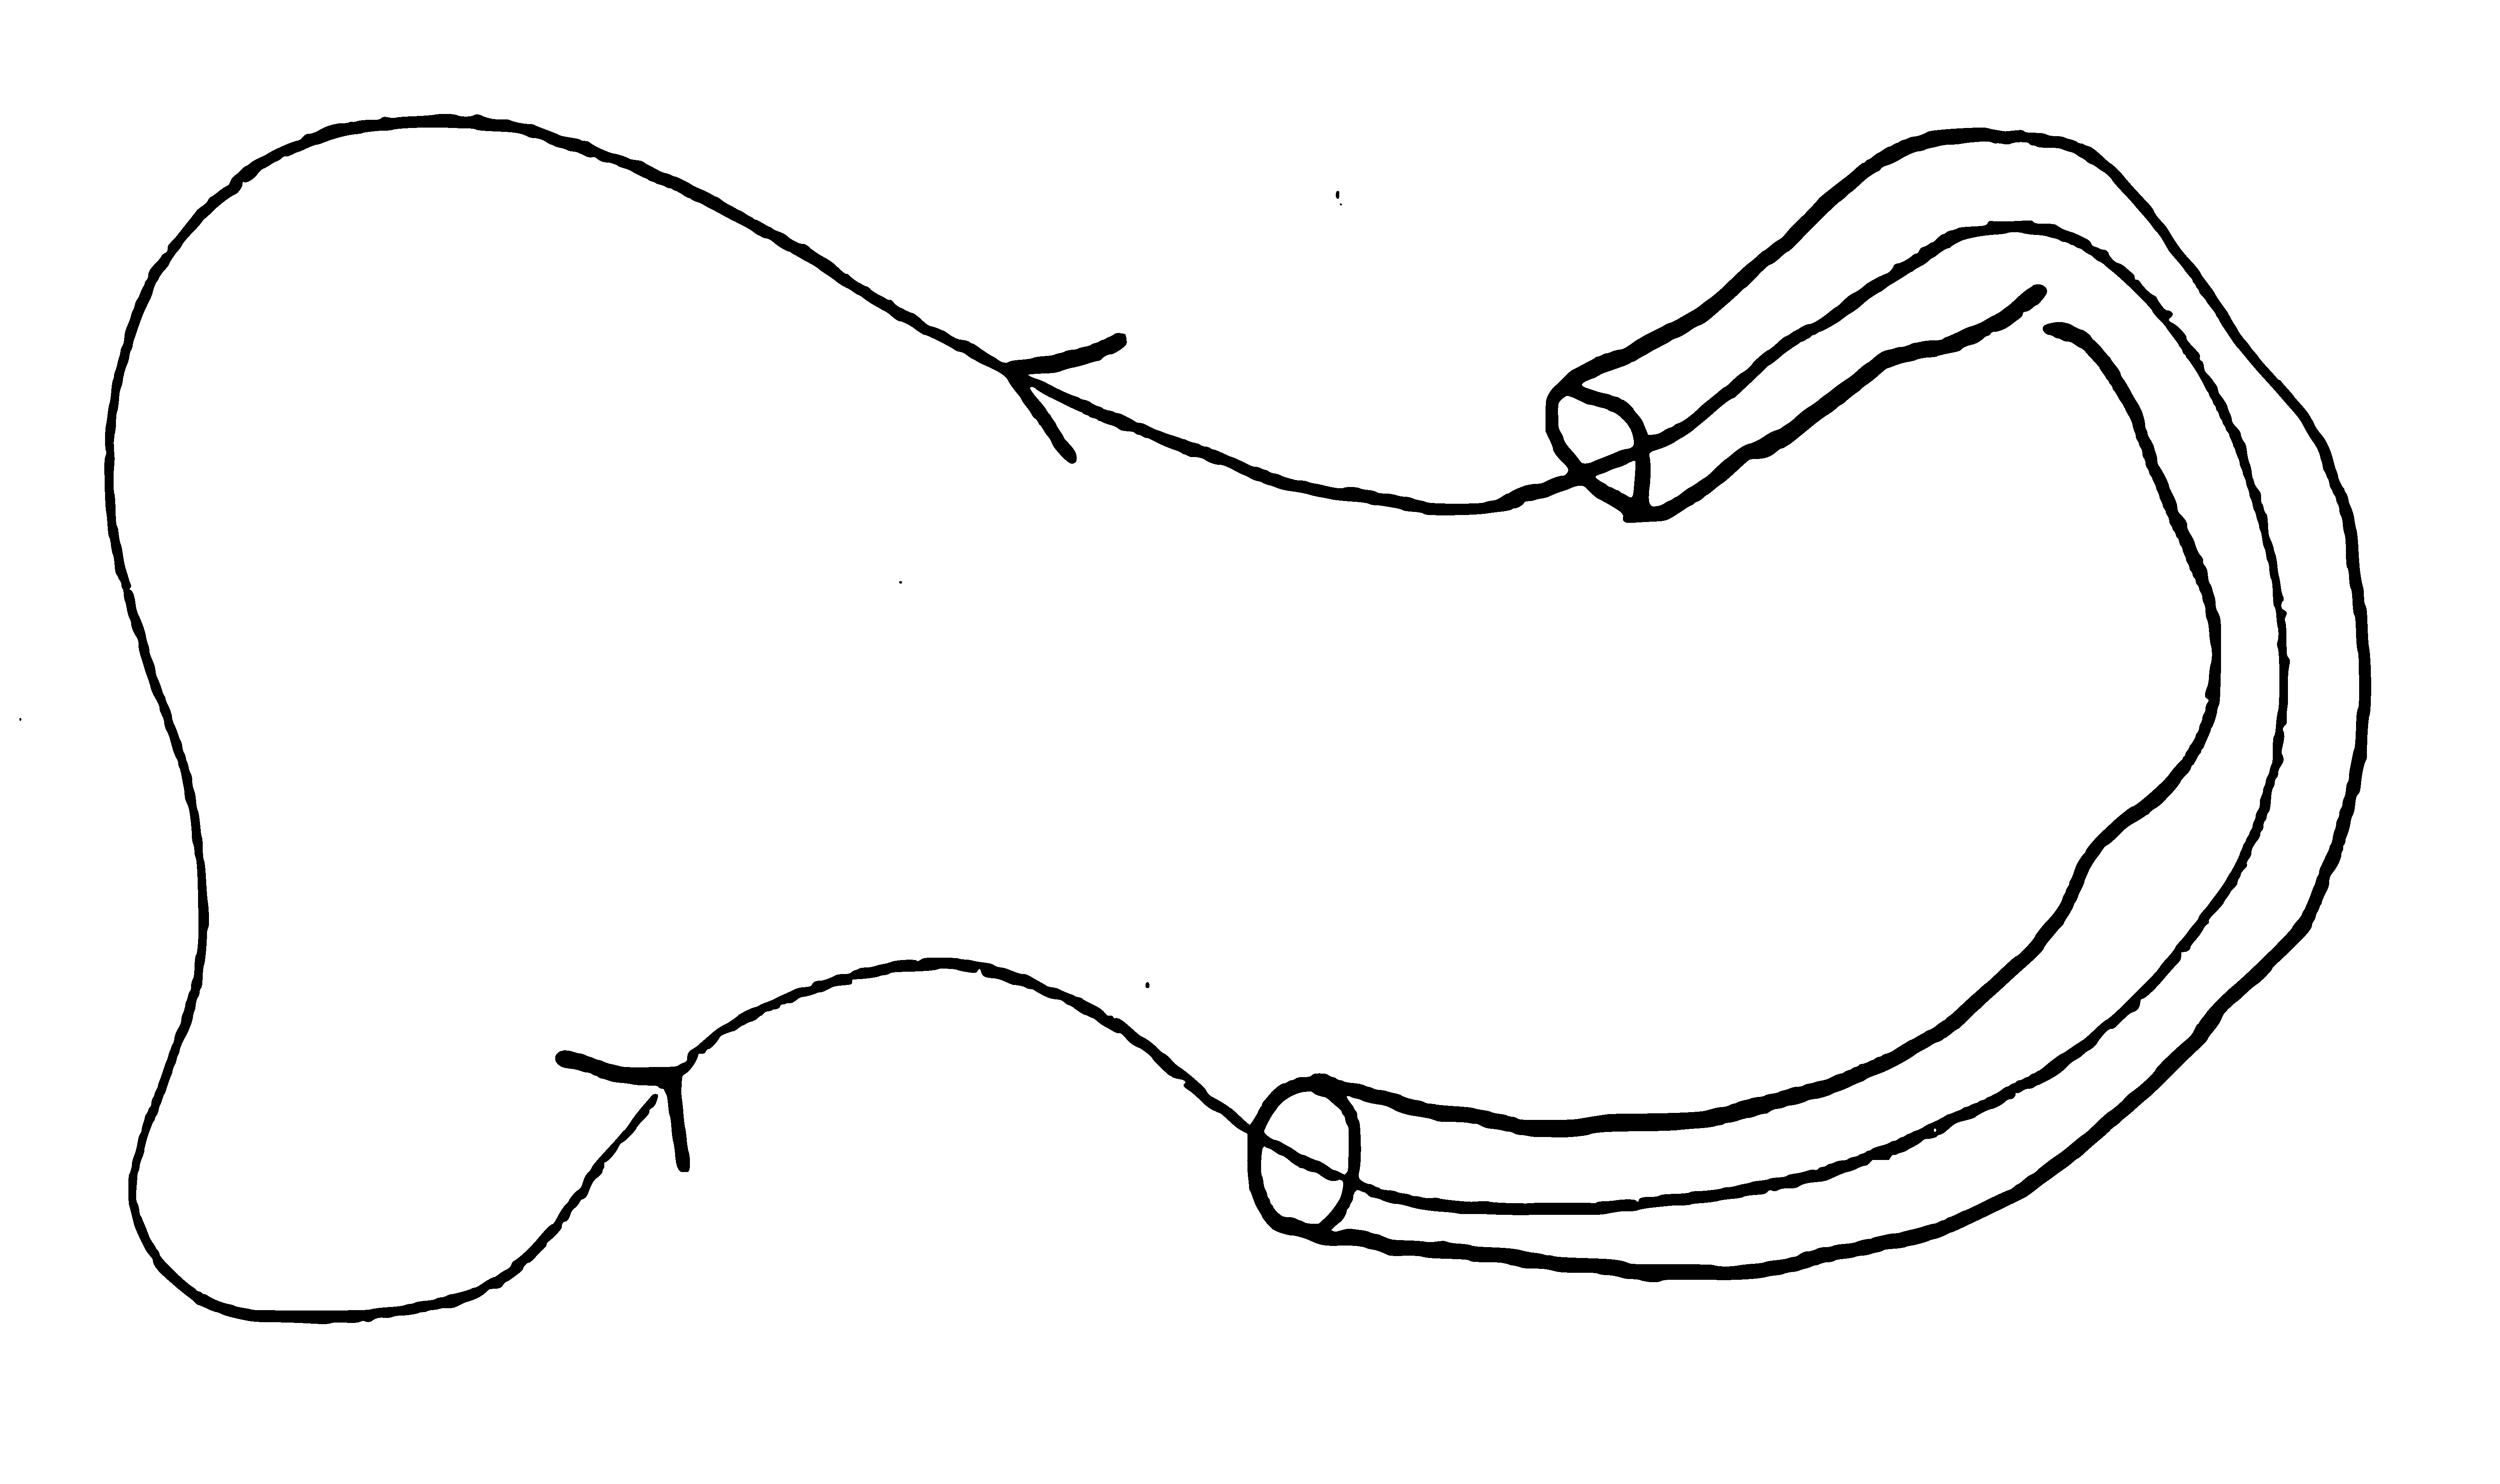
\includegraphics[width=0.5\textwidth]{figures/putkiympäristö.pdf}
    \caption{3-monistoon upotettu suljettu käyrä, jolle piirretty pätkä mielivaltaista putkiympäristöä.}
    \label{kuva:putkiympäristö}
\end{figure}
\begin{lause}[Putkiympäristölause]
    Jokaisella sileän moniston upotetulla sileällä alimonistolla on putkiympäristö.
\end{lause}
\begin{proof}
    Todistus on vaikea ja löytyy lähteestä ???.
\end{proof}
\begin{maaritelma}
    Olkoon $f:\C^2\to\C$ polynomikuvaus. Sen kuitua $f^{-1}(c),c\in\C$ kutsutaan \emph{säännölliseksi}, mikäli jollekin $c$:n ympärisölle $D$ kuvaus $f|_{f^{-1}(D)}:f^{-1}(D)\to D$ on paikallisesti triviaali $C^\infty$-kuidutus.

    Kuitu $f^{-1}(c)$ on \emph{säännöllinen äärettömyydessä}, jos jollekin $c$:n ympäristölle $E$ ja kompaktille osajoukolle $K\subset\C^2$ kuvaus $f|_{f^{-1}(D)-K}$ on paikallisesti triviaali kuidutus. 

    Jos kaikki $f$:n kuidut ovat säännöllisiä äärettömyydessä niin $f$ on \emph{hyvä}.
\end{maaritelma}
\begin{huomautus}
    ``Säännöllinen'' ja ``säännöllinen äärettömyydessä ja epäsingulaarinen'' ovat yhtäpitäviä.
\end{huomautus}
\begin{ajatus}
    Säännöllisyys on matemaattinen muotoilu idealle, että läheiset kuidut ``näyttävät samalta'' kuin $f^{-1}(c)$. Säännöllisyys äärettömyydessä muotoilee tämän samalta näyttämisen äärettömyyden ``lähellä''.
\end{ajatus}

\subsection{Homologiaa pintapuolisesti}
Homologia on sisällöltään rikas ja tekninen matematiikan osa-alue, jonka tarkoituksena on tutkia topologisten avaruuksien rakennetta ja reikiä. Homologian ehtisi tässä työssä esitellä vain lyhyesti, mikä ei tee aihepiirille oikeutta syvyytensä vuoksi; siispä aiheen esittely ohitetaan tässä työssä, mutta kiinnostunutta lukijaa ohjataan tutustumaan erinomaiseen Hatcherin materiaaliin \citep{Hatcher2002}.

Tässä aliosiossa esitetään kuitenkin lyhyt motivaatio homologialle sekä määritellään pari työssä keskeistä käsitettä. Määritelmät tarjoillaan intuitivistisen selityksen kera, homologiaa tuntematonta lukijaa silmälläpitäen.
\begin{ajatus}
    Homologia tutkii topologisten avaruuksien \emph{erilaisuutta} avaruuksien \emph{reikäisyyden} kautta. Reikäisyys on yllättävän vaikeaa määritellä, mutta se auttaa myös yllättävän hyvin erottelemaan avaruuksia toisistaan, esimerkiksi pallon ja toruksen.
\end{ajatus}
\begin{esimerkki}
    Ympyrä $\S^1$ ja kahdeksikko eivät ole homologisia. Ympyrällä sulkee sisäänsä yhden reiän, kahdeksikko kaksi reikää.
\end{esimerkki}
Ympyrän sisäänsä sulkema reikä on tietyssä mielessä kaksiulotteinen. Sitä rajaa yksiulotteinen ympyrä, ja sen paikalle voisi piirtää 2-pinnan. Samaan tapaan on olemassa kolmiulotteisia reikiä. Tällaisen sulkee sisäänsä $\S^2$. Tähän reikään ei voi päästä kolmiulotteisessa avaruudessa käsiksi kulkematta $\S^2$:n pinnan läpi, mutta neljättä ulottuvuutta pitkin reiän läpi voi kulkea koskematta $\S^2$:een.

Käytännössä homologiassa lasketaan homologiaryhmiä $H_n(X)$, missä $X$ on topologinen avaruus. Alaindeksi $n$ kertoo, että kyseessä on $n$:s homologiaryhmä, joka tavallaan mittaa avaruuden $n$-ulotteisia reikiä.
\begin{esimerkki}
    Ympyrälle $\S^1$ homologiaryhmät ovat
    \begin{equation*}
        H_i(\S^1)=
        \begin{cases}
            \Z, & i=0,1 \\
            0, & i>1
        \end{cases}.
    \end{equation*}
    Nollas homologiaryhmä $H_0$ mittaa avaruuden yhtenäisten komponenttien määrää. $H_0(\S^1)=\Z$ tarkoittaa, että ympyröitä voisi olla $k$ kappaletta liimattuna päällekkäin, $k\in\Z$ tai nolla, jos $k=0$.

    $H_1$ mittaa 1-ulotteisten reikien määrää, sitä, montako silmukkaa avaruus tekee yksiulotteisesti.

    $H_n$ mittaa $n$-ulotteisten reikien määrää, mutta $\S^1$:llä ei ole $n$-ulotteisia reikiä.
\end{esimerkki}
\begin{esimerkki}
    Pallon $\S^2$ tapauksessa $H_2(\S^2)=\Z$, mutta $H_1(\S^2)=0$, koska pallon pinnalle piirretyn ympyrän voi aina kiristää pisteeksi, mutta pinnalle asetettua huppua ei voi.
\end{esimerkki}
\begin{esimerkki}
    Toruksella $\T^2=\S^1\times\S^1$ on mielenkiintoisempia ryhmiä:
    \begin{equation*}
        H_i(\T^2)=
        \begin{cases}
            \Z, & i=0,2 \\
            \Z\oplus\Z, & i=1 \\
            0, & i>2
        \end{cases}
    \end{equation*}
    Ryhmä $H_1$ selittyy sillä, että toruksen pinnalle voi piirtää kaksi silmukkaa, joita ei voida muuntaa toisikseen: toruksen ison akselin ympäri, sekä toruksen paksuutta pitkin. Tämä on havainnollistettu kuvassa~\ref{kuva:toruksen-homologia-akselit}
\end{esimerkki}
\begin{figure}
    \centering
    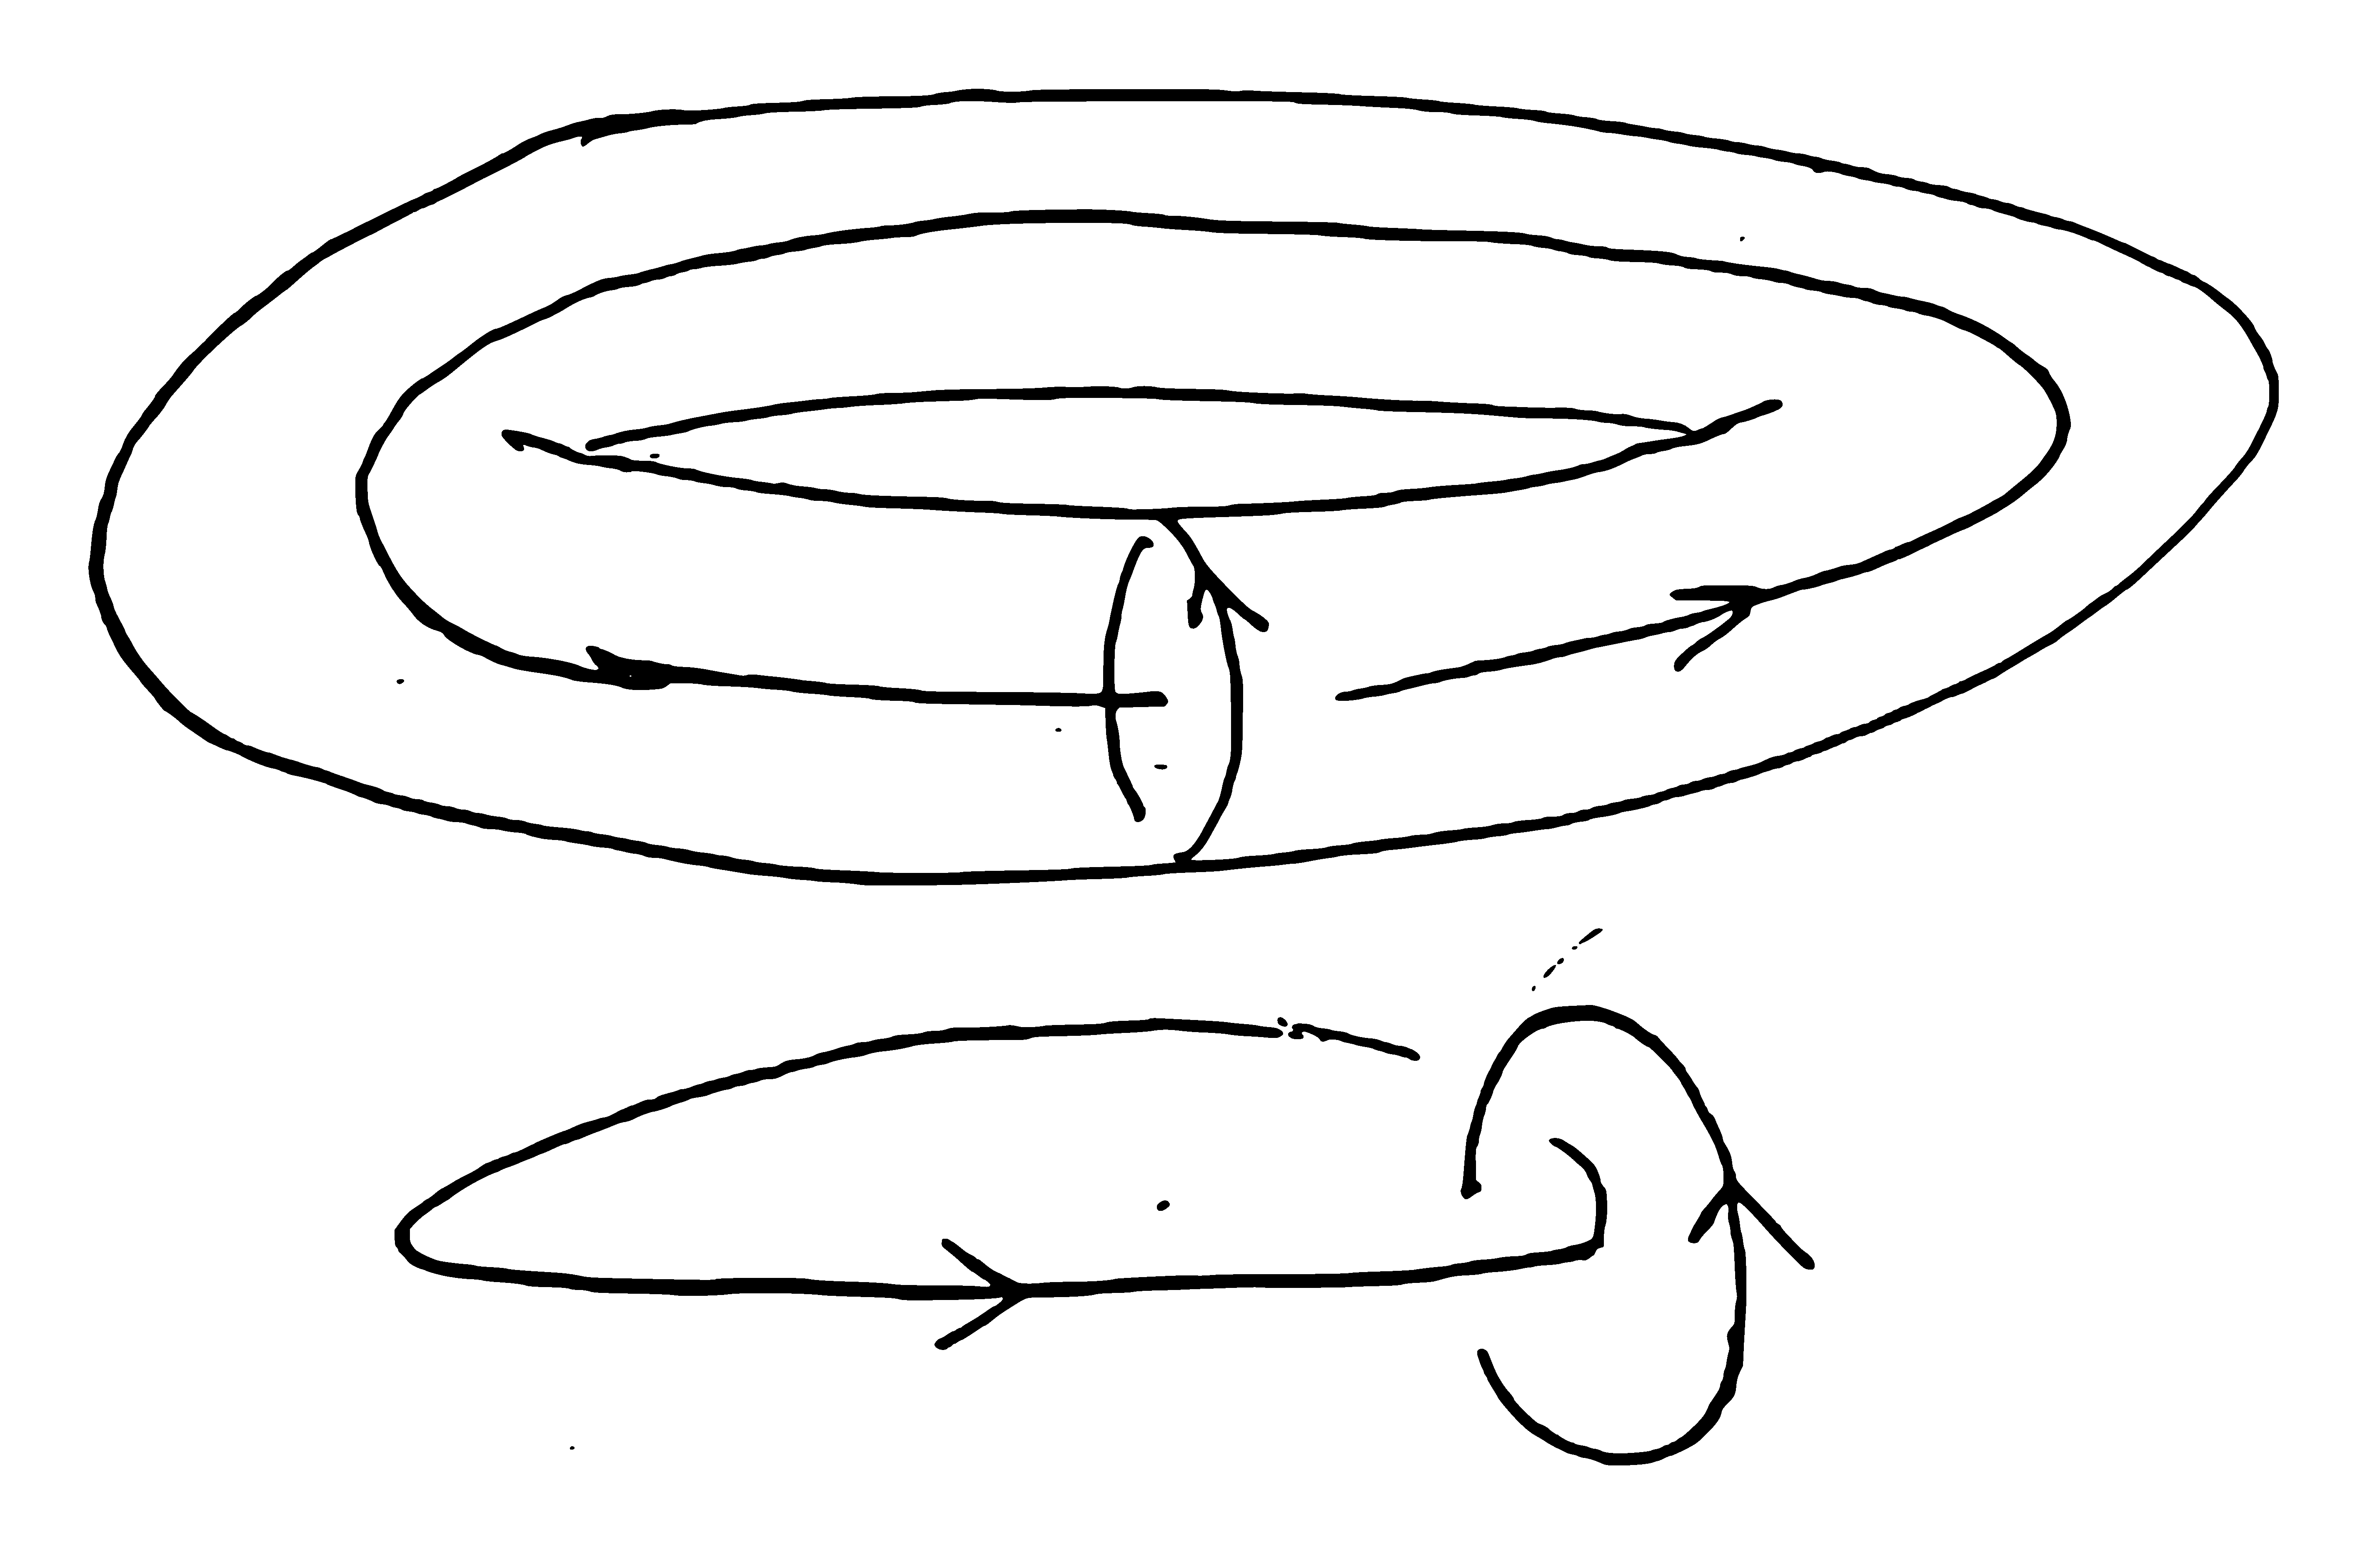
\includegraphics[width=0.5\textwidth]{figures/toruksen-homologia-akselit.pdf}
    \caption{Toruksen kaksi homologia-akselia.}
    \label{kuva:toruksen-homologia-akselit}
\end{figure}
Mitä ympyröiden homologiaryhmiin tulee, lukija saattoi huomata jo kaavaan, joka todistetaan lemmassa~\ref{lemma:ympyröiden-homologia}.
\begin{lemma}
    \label{lemma:ympyröiden-homologia}
    Kaikille $n$-palloille $\S^n$ pätee
    \begin{align*}
        H_0(\S^n)&=H_n(\S^n)=\Z, \\
        H_k(\S^n)&=0,\quad k\ne n.
    \end{align*}
\end{lemma}
\begin{proof}
    Mayer-Vietoris-jono.
\end{proof}
Homologia ei ole kuitenkaan täydellinen keino topologisten avaruuksien erottelemiseksi. On olemassa avaruuksia, jotka eivät ole homeomorfisia, vaikka niiden homologiaryhmät ovat samat kaikilla $n\in\N_0$. Työn kannalta tärkeä yleinen avaruus, jossa työskennellään paljon, on avaruus, joka ainakin homologisesti muistuttaa palloa.
\begin{maaritelma}
    \label{maar:homologinen-n-pallo}
    Topologinen $n$-monisto $X$ on \emph{homologinen $n$-pallo}, jos se tyydyttää lemman~\ref{lemma:ympyröiden-homologia} yhtälöt, ts.
    \begin{align*}
        H_0(X)&=H_n(X)=\Z \\
        H_k(X)&=0,\quad k\ne n
    \end{align*}
\end{maaritelma}

\subsection{Kuidutetut torukset}
Ok ilmeisesti kuidutetut torukset on aika tärkee juttu ja kuidutetut Seifert-monistot (avaruudet?) myös. Tähän tulis selitystä niistä.

\subsection{Homologia (aksiomaattinen yritys)}
Tämä on vähän epätoivoinen yritys sisällyttää homologia työhön. Taidan poistaa koko osion.

Tämän aliosion tarkoitus on kiinnittää työssä käytettävä homologian sanasto. Työn tiivis esitys ei tee oikeutta homologialle ja homologiaa tuntematonta lukijaa suositellaankin sivuuttamaan osio, tai tutustumaan homologiaan Hatcherin kirjan avulla \citep{Hatcher2002}. Aliosio on pikemminkin suunnattu homologiaa tuntevalle lukijalle, joka haluaa varmistaa termistön, tai palata työn myöhemmistä osioista tarkistamaan määritelmiä. Sanastossa noudatetaan kuitenkin yleisiä tapoja, joten myös homologiaa tunteva lukija voi sivuuttaa aliosion.
\begin{maaritelma}
    \emph{CW-kompleksi} on topologinen avaruus $X$, joka muodostetaan algoritmisesti:
    \begin{enumerate}
        \item Valitaan diskreetti joukko $X^0$, jonka alkioita kutsutaan $X$:n \emph{$0$-soluiksi}.
        \item Muodostetaan induktiivisesti \emph{$n$-luuranko $X^n$} $X^{n-1}$:stä liittämällä $n$-soluja $e_\alpha^n$ kuvauksilla $\varphi_\alpha:\pallo^{n-1}\to X^{n-1}$. $X^n$ on tekijä-avaruus
        \begin{equation}
            X^n=\frac{X^{n-1}\sqcup_\alpha D_\alpha^n}{\sim},
        \end{equation}
        missä $\sim$ on relaatio $x\sim\varphi_\alpha(x)$, kun $x\in\partial D_\alpha^n$. Joukon $D_\alpha^n-\partial D_\alpha^n$ kuva tekijäkuvauksen suhteen ja solu $e_\alpha^n$ ja ovat homeomorfisia.
        \item Jatkamalla prosessia saadaan $X=\cup_n X^n$ ja se voidaan varustaa heikolla topologialla: $A\subset X$ on avoin (suljettu) jos ja vain jos $A\cap X^n$ on avoin (suljettu) $X^n$:ssä kaikille $n\in\N$. 
    \end{enumerate}
\end{maaritelma}
\begin{aksiooma}[Homologia-aksioomat]
    \begin{enumerate}
        \item Jos $f\cong g:X\to Y$ niin $f_\bullet=g_\bullet:\tilde h_n(X)\to\tilde h_n(Y)$.
        \item On olemassa reunahomomorfismit $\partial:\tilde h_n(X/A)\to\tilde h_{n-1}(A)$ määritelty kaikille CW-pareille $(X,A)$, siten että jono
        \begin{equation}
            \cdots\xrightarrow{\partial}\tilde h_n(A)\xrightarrow{i_\bullet}\xrightarrow{q_\bullet}\tilde h_n(X/A)\xrightarrow{\partial}\tilde h_n(A)\xrightarrow{i_\bullet}\cdots
        \end{equation}
        on tarkka. Jonossa $i$ on inkluusio ja $q$ tekijäkuvaus.
    \end{enumerate}
\end{aksiooma}
\begin{maaritelma}
    Pelkistetty homologiateoria antaa epätyhjille CW-komplekseille $X$ jonon
    \begin{itemize}
        \item abelisia ryhmiä $\tilde h_n(X)$ ja
        \item homomorfismeja $f_\bullet:\tilde h_n(X)\to\tilde h_n(Y)$ jokaista CW-kompleksien välistä kuvausta $f:X\to Y$ kohden, siten että
        \begin{itemize}
            \item $(fg)_\bullet=f_\bullet g_\bullet$
            \item $\mathbbm{1}_\bullet=\mathbbm{1}$,
        \end{itemize}
    \end{itemize}
    siten, että homologia-aksioomat pitävät.
\end{maaritelma}